\chapter{Weitere Prinzipien} 

\section{Analyse GRASP: Geringe Kopplung}

\subsubsection{Positiv-Beispiel:}

\autoref{fig:coupling-PersistenceWriter} zeigt das Positiv-Beispiel zur geringen Kopplung. \\
Das Interface \textit{ase.application.PersistenceWriter} entkoppelt \textit{ase.application.Game} von 
\textit{ase.plugin.localpersistence.SerializationFilePersistor}. In Game soll es die Möglichkeit geben den aktuellen 
Spielstand zu speichern, damit dieser in Zukunft wieder geladen werden kann und das Spiel fortgesetzt werden kann. 
SerializationFilePersistor bietet diese Möglichkeit, in dem es den aktuellen Spielstand als Java-Objekt serialisiert 
und als Datei im lokalen Dateisystem speichert. Es darf aber auf keinen Fall eine direkte Abhängigkeit von 
Game zu SerializationFilePersistor bestehen, da dies die Dependency Rule brechen würde und außerdem zu einer starken 
Kopplung führen würde. Mit der Abstraktion durch das Interface ist es möglich in Zukunft andere Speichermethoden einzuführen,
ohne dass sich etwas für Game ändert, wodurch sich die positiven Effekte der geringen Kopplung entfalten. 

\begin{figure}[H]
	\centering
	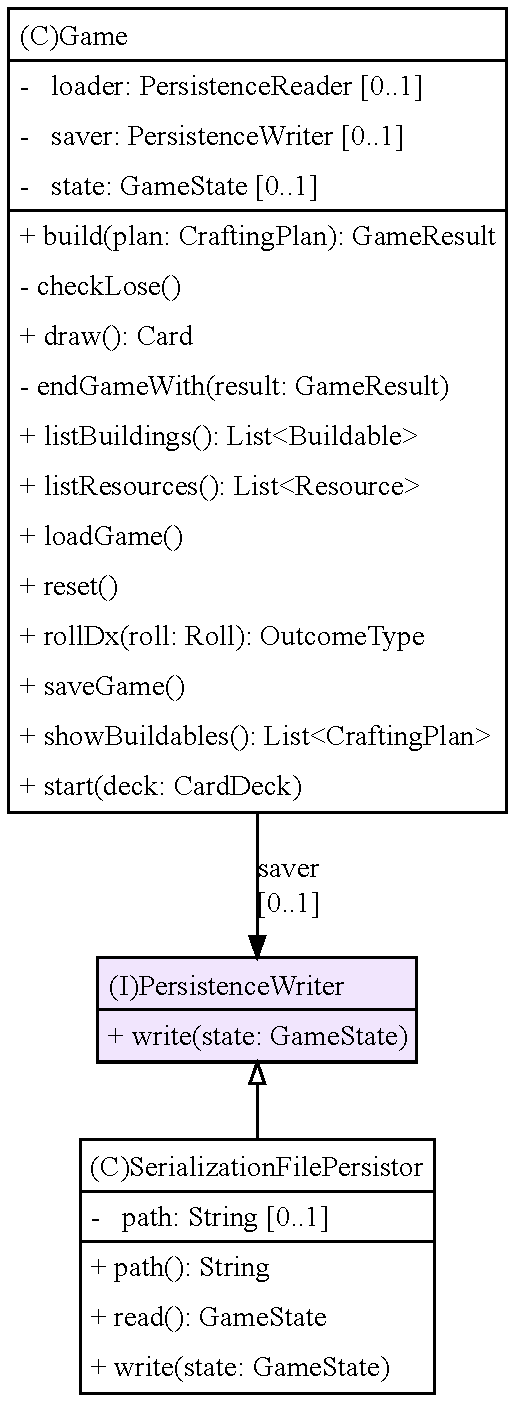
\includegraphics[width=0.5\textwidth]{Bilder/PersistenceWriter_structure.pdf} 
	\caption{UML-Diagramm von \textit{ase.application.PersistenceWriter}.}
	\label{fig:coupling-PersistenceWriter}
\end{figure} 

\subsubsection{Negativ-Beispiel:}

\autoref{fig:coupling-Workbench} zeigt das Negativ-Beispiel, da eine sehr starke Kopplung zwischen \textit{Workbench} 
und \textit{ResourceStash} als direkte Abhängigkeit vorliegt\footnote{Das gleiche Problem besteht auch 
zwischen \textit{Camp} und \textit{Workbench} aber hier wird nur \underline{ein} Negativ-Beispiel gewünscht und behoben.}. \\
Aufgabe der Workbench ist es zu überprüfen, welche \textit{CraftingPlan}s mit den vorhandenen Ressourcen im 
ResourceStash herstellbar sind und Gegenstände mit der \textit{build}-Methode herzustellen, indem dafür die 
nötigen Ressourcen vom ResourceStash verwendet werden. Aufgabe des ResourceStash ist es in erster Linie eine Datenstruktur
zur Lagerung von Ressourcen bereitzustellen. Die Workbench nutzt dabei nur die Methoden \textit{consumeResources} 
und \textit{hasResources} des ResourceStash. \\
Wie \autoref{fig:coupling-Workbench-fixed} zeigt, kann die hohe Kopplung einfach aufgelöst werden, 
indem zwischen Workbench und ResourceStash ein Interface eingezogen wird, welches die Methoden bereitstellt, 
die Workbench zum verichten seiner Aufgaben benötigt. Dadurch könnte in Zukunft ResourceStash mit einer anderen 
Datenstruktur ausgetauscht werden, ohne dass die Workbench davon etwas mitbekommen würde, aufgrund der nun geringen Kopplung.

\begin{figure}[H]
	\centering
	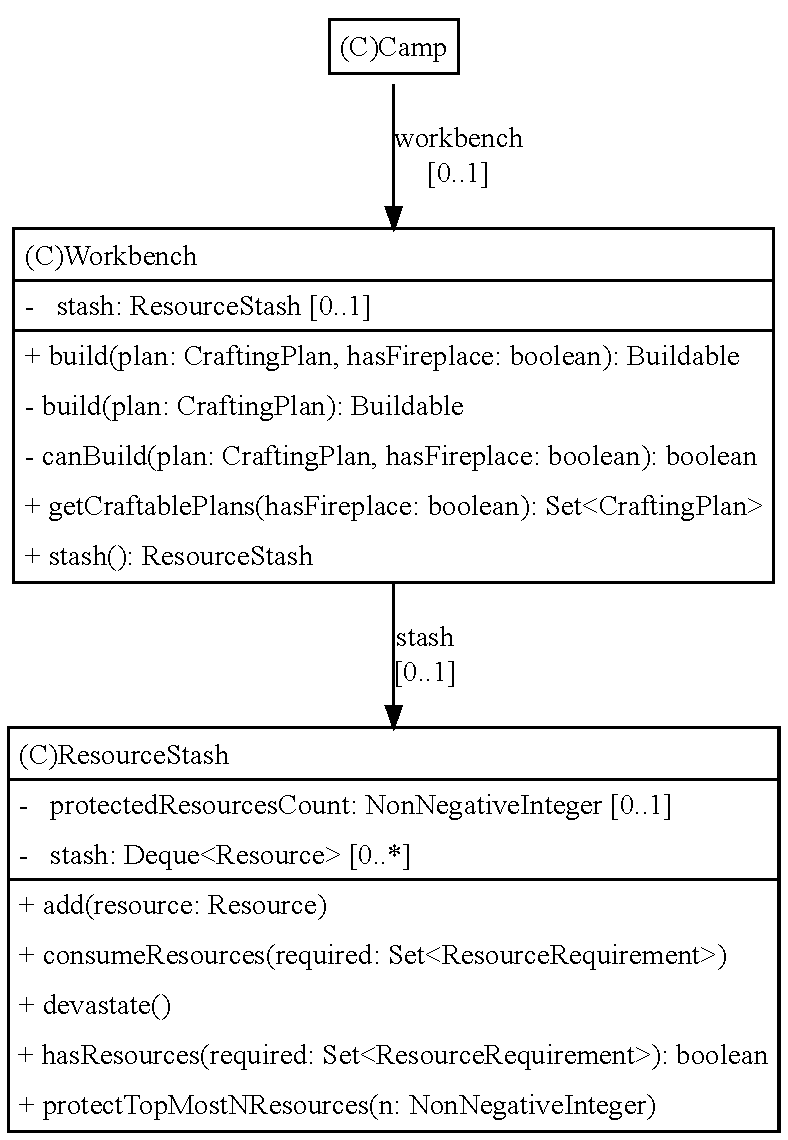
\includegraphics[width=0.5\textwidth]{Bilder/Workbench_structure.pdf} 
	\caption{UML-Diagramm von \textit{ase.domain.crafting.Workbench}.}
	\label{fig:coupling-Workbench}
\end{figure} 

\begin{figure}[H]
	\centering
	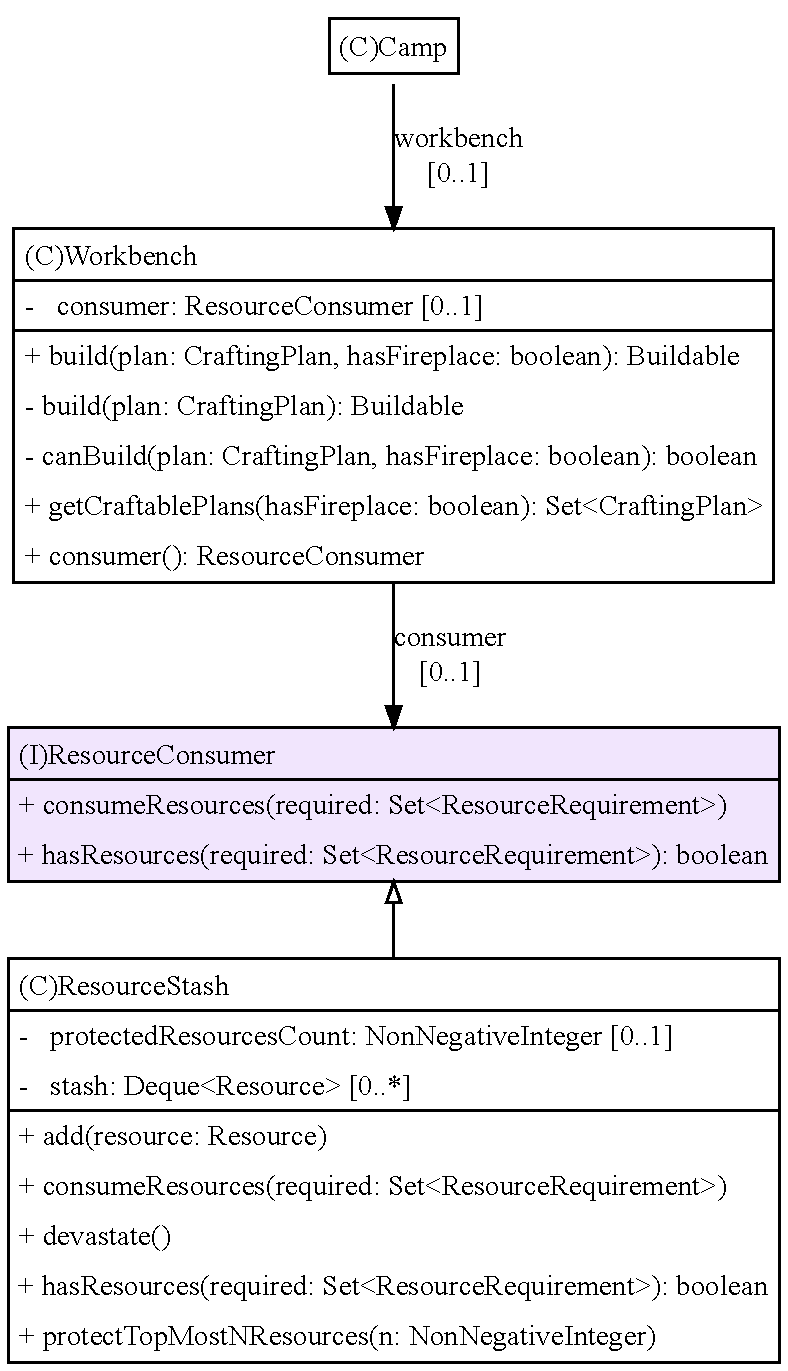
\includegraphics[width=0.5\textwidth]{Bilder/Workbench_fixed_structure.pdf} 
	\caption{\autoref{fig:coupling-Workbench} mit eingezogenem \textit{ResourceConsumer}-Interface 
	zur Auflösung der Kopplung.}
	\label{fig:coupling-Workbench-fixed}
\end{figure} 

\section{Analyse GRASP: Hohe Kohäsion}

\autoref{fig:cohesion-ResourceRequirement} zeigt das UML-Diagramm der Klasse \textit{ResourceRequirement}, 
welches eine sehr hohe Kohäsion hat. Es handelt sich um ein Datentupel aus (Ressource, Menge), 
welches im \textit{CraftingPlan}-Enum verwendet wird, um die benötigten Ressourcen für das jeweilige 
Buildable anzugeben. Die Kohäsion ist sehr hoch, da zu einer Bedarfsangabe immer gehört, welcher Gegenstand 
(\textit{resource}) benötigt wird und wie viel davon (\textit{amount}). Die beiden Angaben sind im Rahmen der 
Bedarfsangabe semantisch maximal zusammenhängend und können inhaltlich nicht voneinander getrennt werden.   

\begin{figure}[H]
	\centering
	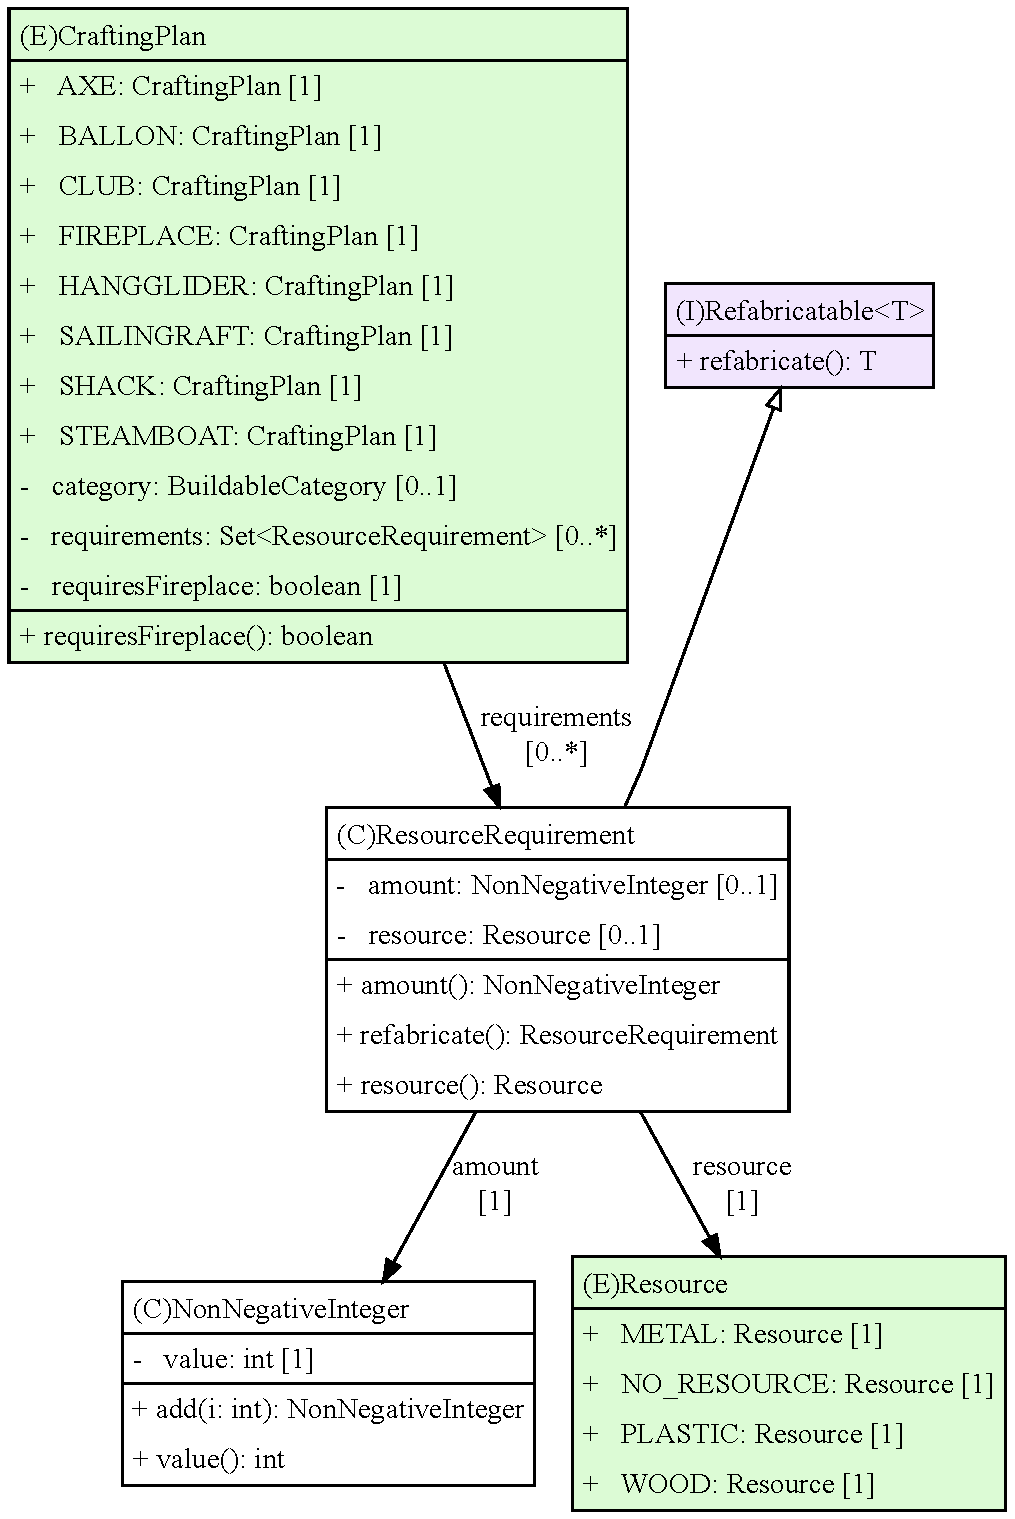
\includegraphics[width=0.55\textwidth]{Bilder/ResourceRequirement_structure.pdf} 
	\caption{UML-Diagramm von \textit{ase.domain.crafting.ResourceRequirement}.}
	\label{fig:cohesion-ResourceRequirement}
\end{figure} 


\section{Don't Repeat Yourself (DRY)}

In Commit \texttt{e246d77b} wurde der folgende duplizierte Code aus der \textit{Game}-Klasse gebündelt: \\
\texttt{state.setPhase(GamePhase.END);} \\
\texttt{state.setStatus(GameStatus.ENDED);} \\
\texttt{state.setResult(X);} \\
\autoref{code:dry-before} zeigt den Code ein Commit vorher (ID: \texttt{b4399813}).
\autoref{code:dry-after} zeig den Code mit der neuen Methode \textit{endGameWith}, die die das Code-Duplikat 
an allen drei Stellen entfernt. \\
Es ist wichtig den Code an der Stelle anzupassen, um bei Änderungen der Game-Schlusslogik, keine 
Stelle ausversehen zu vergessen, was zu Bugs führen könnte. Ein Beispiel wäre, dass ein zusätzlicher Zustand 
gesetzt werden muss, Observern ein Statusupdate mitgeteilt werden soll, oder ein anderer Zustand gesetzt 
werden soll, weil sich das Modell ändert. \\
Durch das Entfernen der Duplikate ist der Code kürzer, einfacher, besser lesbar (sprechender Name der Methode anstatt 
willkürlich erscheinende Statusänderungen) und besser wartbar aus den zuvor genannten Gründen.   


\lstinputlisting[
	label=code:dry-before,    % Label; genutzt für Referenzen auf dieses Code-Beispiel
	caption=DRY-Code der \textit{Game}-Klasse zum Commit \texttt{b4399813}.,
	captionpos=b,               % Position, an der die Caption angezeigt wird t(op) oder b(ottom)
	style=EigenerJavaStyle,   % Eigener Style der vor dem Dokument festgelegt wurde
	firstline=1,                % Zeilennummer im Dokument welche als erste angezeigt wird
	lastline=100                 % Letzte Zeile welche ins LaTeX Dokument übernommen wird
]{Quellcode/dry-before.java}

\lstinputlisting[
	label=code:dry-after,    % Label; genutzt für Referenzen auf dieses Code-Beispiel
	caption=DRY-Code der \textit{Game}-Klasse zum Commit \texttt{e246d77b}.,
	captionpos=b,               % Position, an der die Caption angezeigt wird t(op) oder b(ottom)
	style=EigenerJavaStyle,   % Eigener Style der vor dem Dokument festgelegt wurde
	firstline=1,                % Zeilennummer im Dokument welche als erste angezeigt wird
	lastline=100                 % Letzte Zeile welche ins LaTeX Dokument übernommen wird
]{Quellcode/dry-after.java}


